\chapter{Metodolog\'ia y dise\~no de un m\'etodo para inducir ansiedad en cuidadores de personas con demencia}\label{capit:cap3}
\vspace{-2.0325ex}%
\noindent
\rule{\textwidth}{0.5pt}
\vspace{-5.5ex}% 
\newcommand{\pushline}{\Indp}% Indent puede ir o no :p
\section{Introducci\'on}\label{secc:introduction}

Como vimos en el cap\'itulo 2, la mayor\'ia de los estudios logran inducir ansiedad o estr\'es por medio de situaciones controladas dentro del laboratorio exitosamente. Sin embargo, generar ansiedad en cuidadores informales es mucho mas dif\'icil: El escenario de un laboratorio no coincide con el entorno en el que una persona con demencia se desarrolla por lo que los comportamientos impredecibles no ser\'ian congruentes con el ambiente. Adem\'as, exponer a personas sin experiencia ante una persona con demencia que tiene necesidades reales resultar\'ia riesgoso para ambos individuos. Por otra parte, realizar una intervenci\'on totalmente natural a\~nade un grado de dificultad al estudio, resultando en ruido en los datos recolectados (p. ej. la se\~nal de ritmo card\'iaco podr\'ia ser alta no por una situaci\'on de ansiedad, sino por una actividad f\'isica, m\'ultiples distracciones o responsabilidades al mismo tiempo para el cuidador) haciendo d\'ificil de analizarlos para probar hip\'otesis.

A continuaci\'on, se muestra un experimento que implementa la  t\'ecnica conocida como ``Naturalistic enactment (NE)'' \cite{Castro11}


\section{Un experimento para inducir ansiedad en cuidadores informales}
\begin{figure}[h]
        \centering
        \subfigure[]{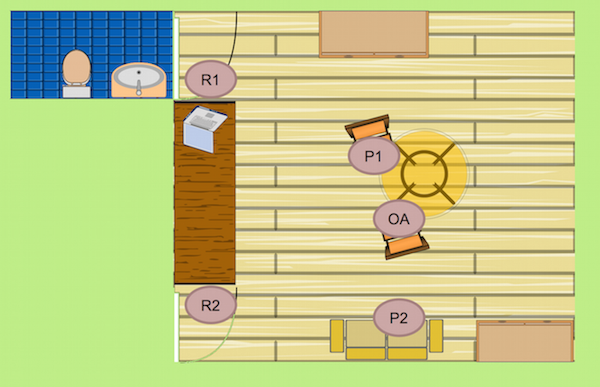
\includegraphics[width=160mm,height=80mm]{./Figures/img_exp_setup}}
        \caption{Configuraci\'on del escenario del experimento} \label{fig:img_exp_setup}
\end{figure}

\newpage
%%=====================================================

